\documentclass[../main.tex]{subfiles}
\begin{document}
$n$维欧几里得空间$\mathcal{E}$中的一个点$X\in\mathcal{E}$,只有在选择了某一恰当的坐标系后,才可唯一对应于一个有序实数$n$元组$\left(x_1,\cdots,x_n\right)\in\mathbb{R}^n$,作为这个点在这一个坐标系下的坐标。如果所选择的是直角坐标系,那么点$X$的坐标是它的位置向量在$\mathcal{E}$的平移空间$\mathcal{V}_\mathcal{E}$的一组规范正交基下的坐标。但是,我们还可以在同一个欧几里得空间中建立各种曲线坐标系。我们将会看到,在曲线坐标系下,$X$仍可唯一对应于一个有序实数$n$元组,但曲线坐标系下的坐标与直角坐标系下的坐标之间的变换法则,并非向量空间下的基变换规律。因此,仅按\S\ref{sec:II.2.3}知识是无法解决的。

正式地,设$\mathcal{E}$是一个$n$维欧几里得空间,$\mathcal{V}_\mathcal{E}$是$\mathcal{E}$的平移空间,$\mathcal{E}$的基本直角坐标系是$\left(O,\left\{\mathbf{\hat{e}}_i\right\}\right)$,$\mathcal{E}$中的每个点$X\in\mathcal{E}$就已经唯一地对应$\mathbb{R}^n$中的一个元素$\left(x_1,\cdots,x_n\right)$作为它在这个直角坐标系下的坐标。一个恰当地建立的\emph{曲线坐标系(curvilinear coordinate system)},也能使$\mathcal{E}$中的每个点$X$唯一地对应于$\mathbb{R}^n$中的一个元素$\left(u_1,\cdots,u_n\right)\in\mathbb{R}^n$,作为它在这个曲线坐标系下的坐标。在直角坐标系,从$\mathcal{E}$到$\mathbb{R}^n$的对应关系是双射。而一个恰当的曲线坐标系,首先应能保证每个$X\in\mathcal{E}$都能唯一对应一个不同的$\left(u_1,\cdots,u_n\right)\in\mathbb{R}^n$(单射),但就不一定是一个满射了。我们把曲线坐标系下,所有欧几里得空间的点的坐标的集合记为$\mathcal{U}\subseteq\mathbb{R}^n$,称为\emph{曲线坐标系的参数域}。直角坐标系作为一个特殊的曲线坐标系,它的参数域$\mathcal{U}=\mathbb{R}^n$。设由$\mathcal{U}$到$\mathbb{R}^n$的双射$T:\mathbb{R}^n\supset\mathcal{U}\rightarrow\mathbb{R}^n$把同一个点$X\in\mathcal{E}$的曲线坐标$\left(u_1,\cdots,u_n\right)\in\mathcal{U}$映射其原点相同的直角坐标系下的坐标$\left(x_1,\cdots,x_n\right)\in\mathbb{R}^n$。我们不失一般性地再规定,我们所讨论的任一曲线坐标系的映射$T$是至少一阶连续可微的。例\ref{ex:II.6.1}以我们以前所熟悉的3维欧几里得空间下的柱坐标系和球坐标系为例,给出了这两个曲线坐标系下的映射$T$。请注意为了保证$T$的双射性所做的仔细讨论。

\begin{figure}[h]
    \centering
    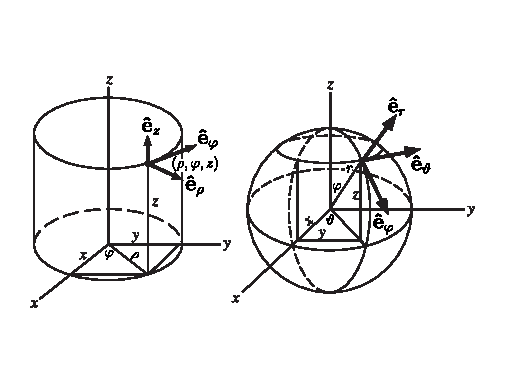
\includegraphics[width=0.75\textwidth]{images/cylindrical_spherical_coordinate_basis.pdf}
    \caption{柱坐标系和球坐标系的基和几何图象}
    \label{fig:II.5.2}
\end{figure}

\begin{example}[柱坐标系与球坐标系的参数域映射]\label{exp:II.5.1}
    设$\mathcal{E}$是3维欧几里得空间,$O\in\mathcal{E}$是选定的原点。记任一点$X$的直角坐标系坐标是$\left(x,y,z\right)$,柱坐标系(cylindrical coordinate system)的坐标是$\left(\rho,\varphi,z\right)$,球坐标系(spherical coordinate system)的坐标是$\left(r,\vartheta,\varphi\right)$(图\ref{fig:II.5.2})。

    记柱坐标系的参数域$\mathcal{U}_\mathrm{cyl}=\left\{\left(\rho,\varphi,z\right)\in\mathbb{R}^3|\rho\geq 0,\varphi\in\left[0,2\pi\right),z\in\mathbb{R}\right\}$,可定义映射$T_\mathrm{cyl}:\mathcal{U}_\mathrm{cyl}\rightarrow\mathbb{R}^3$,
    \[\left(x,y,z\right)=T_\mathrm{cyl}\left(\rho,\varphi,z\right)=\left\{\begin{array}{ll}
            \left(\rho\cos\varphi,\rho\sin\varphi,z\right), & \rho>0 \\\left(0,0,0\right),&\rho=0\end{array}\right.\]

    $T_\mathrm{cyl}$是双射,简单证明如下。若$\rho\neq 0$且$T_\mathrm{cyl}\left(\rho,\varphi,z\right)=T_\mathrm{cyl}\left(\rho^\prime,\varphi^\prime,z\right)$,则有$\tan\varphi=\tan\varphi^\prime$,即$\varphi=\varphi^\prime$或$\varphi=\varphi^\prime+\pi$。易知当$\varphi=\varphi^\prime+\pi$时$\rho=\rho^\prime=0$,与假设矛盾, 故有且仅有$\varphi=\varphi^\prime$。若$\rho=0$,则$\varphi=0$,按条件有且仅有$\rho^\prime=0$且$\varphi^\prime=0$。因此$T_\mathrm{cyl}$是单射。若$\left(x,y\right)\neq\left(0,0\right)$,则只要令$\rho=\sqrt{x^2+y^2}$,$\varphi=\mathrm{atan2}\left(x,y\right)$,即可得到$\left(x,y\right)=T_\mathrm{cyl}\left(\rho,\varphi,z\right)$;当$\left(x,y\right)=\left(0,0\right)$时,只要令$\rho=\sqrt{x^2+y^2}$,$\varphi=0$,即可得到$\left(x,y\right)=T_\mathrm{cyl}\left(\rho,\varphi,z\right)$。因此$T_\mathrm{cyl}$是满射。因此$T_\mathrm{cyl}$是双射。

    上一段出现的\emph{双变量反正切函数}$\mathrm{atan2}:\mathbb{R}^2\setminus\left\{(0,0)\right\}\rightarrow\left[0,2\pi\right)$,是一个常用的函数,定义为
    \[\mathrm{atan2}\left(x,y\right)=\left\{\begin{array}{ll}
            \mathrm{Arctan}\left(\frac{x}{y}\right),      & y>0,x\geq 0 \\
            \mathrm{Arctan}\left(\frac{x}{y}\right)+2\pi, & y>0,x<0     \\
            \mathrm{Arctan}\left(\frac{x}{y}\right)+\pi,  & y<0         \\
            \frac{\pi}{2},                                & y=0,x>0     \\
            \frac{3\pi}{2},                               & y=0,x<0
        \end{array}\right.
    \]
    其中$\mathrm{Arctan}$表示反正切主值函数,其值域是$\left(-\frac{\pi}{2},\frac{\pi}{2}\right)$。$T_\mathrm{cyl}$的逆映射$T_\mathrm{cyl}^{-1}$可表示为
    \[\left(\rho,\varphi,z\right)=T^{-1}\left(x,y,z\right)=\left\{\begin{array}{ll}
            \left(\sqrt{x^2+y^2},\mathrm{atan2}\left(x,y\right),z\right), & \left(x,y\right)\neq\left(0,0\right) \\
            \left(0,0,z\right),                                           & \left(x,y\right)=\left(0,0\right)
        \end{array}\right.
    \]

    记球坐标系的参数域$\mathcal{U}_\mathrm{sph}=\left\{\left(r,\vartheta,\varphi\right)\in\mathbb{R}^3 \mid r\geq 0,\vartheta\in\left[0,2\pi\right),\varphi\in\left[0,\pi\right]\right\}$,可定义映射$T_\mathrm{sph}:\mathcal{U}_\mathrm{sph}\rightarrow\mathbb{R}^3$,
    \[
        \left(x,y,z\right)=T_\mathrm{sph}\left(r,\vartheta,\varphi\right)=\left\{\begin{array}{ll}

            \left(r\sin\vartheta\cos\varphi,r\sin\vartheta\sin\varphi,r\cos\vartheta\right), & r>0 \\
            \left(0,0,0\right),                                                              & r=0
        \end{array}\right.
    \]
    用类似之前的方法可证明$T_\mathrm{sph}$是双射,需且只需取其逆映射为
    \[
        \begin{aligned}
            \left(r,\vartheta,\varphi\right) & =T^{-1}_\mathrm{sph}\left(x,y,z\right)                                                                                                                                         \\
                                             & =\left\{\begin{array}{ll}
                                                           \left(\sqrt{x^2+y^2+z^2},\mathrm{atan2}\left(x,y\right),\mathrm{Arccos}\left(\frac{z}{\sqrt{x^2+y^2+z^2}}\right)\right), & \left(x,y\right)\neq \left(0,0\right) \\
                                                           \left(0,0,0\right),                                                                                                      & \left(x,y\right)=\left(0,0\right)
                                                       \end{array}\right.
        \end{aligned}
    \]

    还可以证明的是,$T_\mathrm{cyl}$和$T_\mathrm{sph}$在它们的定义域上处处都是一阶连续可微的。
\end{example}

记$T$的雅可比矩阵是
\[J\equiv\left(\mathrm{D}T\right)=\left(\begin{array}{ccc}
            \frac{\partial x_1}{\partial u_1} & \cdots & \frac{\partial x_1}{\partial u_n} \\
            \vdots                            & \ddots & \vdots                            \\
            \frac{\partial x_n}{\partial u_1} & \cdots & \frac{\partial x_n}{\partial u_n}
        \end{array}\right)\]
由于$T$是双射且连续可微,由反函数定理\ref{thm:II.4.12},$J$是可逆的,其各列之间线性无关。记以$J$各列作为基$\left\{\mathbf{\hat{e}}_i\right\}$下的坐标的$\mathcal{V}_\mathcal{E}$中的向量为$\mathbf{c}_i,i=1,\cdots,n$,即$\mathbf{c}_i=\sum_{j=1}^n J_{ij}\mathbf{\hat{e}}_j=\sum_{j=1}^n\partial x_j/\partial u_i\mathbf{\hat{e}}_j,i=1,\cdots,n$。则$\left\{\mathbf{c}_i\right\}$是$\mathcal{V}_\mathcal{E}$线性无关向量组,那么它就是$\mathcal{V}_\mathcal{E}$的基。$\left\{\mathbf{\hat{c}}_i\right\},\mathbf{\hat{c}}_i=\mathbf{c}_i/\left\|\mathbf{c}_i\right\|,i=1,\cdots,n$就是$\mathcal{V}_\mathcal{E}$的规范正交基。我们把$\left\{\mathbf{\hat{c}}_i\right\}$称为\emph{曲线坐标系的基},把$h_i=\left\|\mathbf{c}_i\right\|^{-1}$称为曲线坐标系的\emph{拉梅系数(Lam\'{e} coefficients)}。如果$\left\{\mathbf{\hat{c}}_i\right\}$两两正交,那么这个曲线坐标系称为\emph{正交曲线坐标系(orthogonal curvilinear coodinate)}。曲线坐标系的基的内积$g_{ij}=\left(\mathbf{c}_i\mid\mathbf{c}_j\right),i,j=1,\cdots,n$称为该曲线坐标系的\emph{度量张量(metrix tensor)},虽称为张量,但其实$g_{ij}$只是组成了一个对称矩阵。特别地,对于直角坐标系,$g_{ij}=\delta_{ij}$。

在这里需要注意两件事。第一,我们所讨论的映射$T$是关于同一个点$X$的坐标之间的映射,一般地偏导数$\partial x_j/\partial u_i$依赖点$X$的变化而变化,因此$\left\{\mathbf{\hat{c}}_i\right\}$不是$\mathcal{V}_\mathcal{E}$的常向量基。同理$h_i$也是点$X$的函数。第二,虽然点$X$在直角坐标系下的坐标$\left(x_1,\cdots,x_n\right)$恰好满足$\mathbf{r}_X=\sum_{i=1}^nx_i\mathbf{\hat{e}}_i$,但其在曲线坐系下的坐标$\left(u_1,\cdots,u_n\right)$一般不满足$\mathbf{r}_X=\sum_{i=1}^nu_i\mathbf{\hat{c}}_i$。这是因为映射$T$一般不是线性的。作为一般讨论,我们记点$X$在曲线坐标系的基下的坐标为$\left(x_1^\mathrm{c},\cdots,x_n^\mathrm{c}\right)$,即$\mathbf{r}_X=\sum_{i=1}^nx_i^\mathrm{c}\mathbf{\hat{c}}_i$。在每个点$X$处,仍然可以使用基变换与坐标变换公式来联系$\left(x_1,\cdots,x_n\right)$和$\left(x_1^\mathrm{c},\cdots,x_n^\mathrm{c}\right)$。记由$\left\{\mathbf{\hat{e}}_i\right\}$到$\left\{\mathbf{\hat{c}}_i\right\}$的过渡矩阵是$S$,则基变换公式是
\[
    \begin{aligned}
        \mathbf{\hat{c}}_i & =\sum_{j}S_{ji}\mathbf{\hat{e}}_j,                               \\
        \mathbf{\hat{e}}_i & =\sum_j S_{ji}^\mathrm{inv}\mathbf{\hat{c}}_j,\quad i=1,\cdots n
    \end{aligned}
\]
与$\mathbf{\hat{c}}_i$的表达式比较,可知
\[S_{ij}=h_j^{-1}\frac{\partial x_i}{\partial u_j},\quad i,j=1,\cdots,n\]
即矩阵$S$也是依赖点$X$变化的。坐标变换公式是
\[
    \begin{aligned}
        x_i            & =\sum_j S_{ij}x_j^\mathrm{c},                    \\
        x_i^\mathrm{c} & =\sum_jS_{ij}^\mathrm{inv}x_j,\quad i=1,\cdots,n
    \end{aligned}
\]

\begin{example}[柱坐标系和球坐标系的基]\label{exp:II.5.2}
    $T_\mathrm{cyl}$的雅可比矩阵是$J_\mathrm{cyl}$是
    \[
        J_\mathrm{cyl}=\left(\begin{array}{ccc}
                \cos\varphi & -\rho\sin\varphi & 0 \\
                \sin\varphi & \rho\cos\varphi  & 0 \\
                0           & 0                & 1
            \end{array}\right)
    \]
    柱坐标的拉梅系数是$h_\rho=1,h_\varphi=\rho,h_z=1$。过渡矩阵$S_\mathrm{cyl}$是
    \[
        S_\mathrm{cyl}=\left(\begin{array}{ccc}\cos\varphi & -\sin\varphi & 0 \\
             \sin\varphi      & \cos\varphi  & 0 \\
             0                & 0            & 1\end{array}\right)
    \]
    柱坐标的基与直角坐标系的基的关系是
    \[
        \begin{aligned}
            \mathbf{\hat{e}}_\rho    & =\cos\varphi\mathbf{\hat{e}}_x+\sin\varphi\mathbf{\hat{e}}_y,  \\
            \mathbf{\hat{e}}_\varphi & =-\sin\varphi\mathbf{\hat{e}}_x+\cos\varphi\mathbf{\hat{e}}_y, \\
            \mathbf{\hat{e}}_z       & =\mathbf{\hat{e}}_z
        \end{aligned}
    \]
    位置向量在柱坐标系的基下的坐标是
    \[\mathbf{r}_X=\rho\mathbf{\hat{e}}_\rho+z\mathbf{\hat{e}}_z\]
    我们发现,位置向量在$\mathbf{\hat{e}}_\varphi$方向上的投影总是零。诚然,如图\ref{fig:II.5.2}所示,$\mathbf{r}_X$总是与$\mathbf{\hat{e}}_\varphi$正交的。

    $T_\mathrm{sph}$的雅可比矩阵是$J_\mathrm{sph}$是
    \[
        J_\mathrm{sph}=\left(\begin{array}{ccc}
                \sin\vartheta\cos\varphi & r\cos\vartheta\cos\varphi & -r\sin\vartheta\sin\varphi \\
                \sin\vartheta\sin\varphi & r\cos\vartheta\sin\varphi & r\sin\vartheta\cos\varphi  \\
                \cos\vartheta            & -r\sin\vartheta           & 0
            \end{array}\right)
    \]
    球坐标的拉梅系数是$h_r=1,h_\vartheta=r,h_\varphi=r\sin\vartheta$。过渡矩阵是
    \[
        S_\mathrm{sph}=\left(\begin{array}{ccc}
                \sin\vartheta\cos\varphi & \cos\vartheta\cos\varphi & -\sin\varphi \\
                \sin\vartheta\sin\varphi & \cos\vartheta\sin\varphi & \cos\varphi  \\
                \cos\vartheta            & -\sin\vartheta           & 0
            \end{array}\right)
    \]
    球坐标的基与直角坐标系的基的关系是
    \[
        \begin{aligned}
            \mathbf{\hat{e}}_r         & =\sin\vartheta\cos\varphi\mathbf{\hat{e}}_x+\sin\vartheta\sin\varphi\mathbf{\hat{e}}_y+\cos\vartheta\mathbf{\hat{e}}_z, \\
            \mathbf{\hat{e}}_\vartheta & =\cos\vartheta\cos\varphi\mathbf{\hat{e}}_x+\cos\vartheta\sin\varphi\mathbf{\hat{e}}_y-\sin\vartheta\mathbf{\hat{e}}_z, \\
            \mathbf{\hat{e}}_\varphi   & =-\sin\varphi\mathbf{\hat{e}}_x+\cos\varphi\mathbf{\hat{e}}_y
        \end{aligned}
    \]
    位置向量在球坐标系的基下的坐标是
    \[
        \mathbf{r}_X=r\mathbf{\hat{e}}_r
    \]
    我们发现,位置向量在$\mathbf{\hat{e}}_\vartheta$和$\mathbf{\hat{e}}_\varphi$方向上的投影总是零。诚然,如图\ref{fig:II.5.2}所示,$\mathbf{r}_X$总是与$\mathbf{\hat{e}}_\vartheta$和$\mathbf{\hat{e}}_\varphi$正交的。
\end{example}



%=============================
% \section{场函数的导数}
% 设$f:\mathcal{D}\supseteq\mathcal{N}\rightarrow\mathcal{F}$是定义在$\mathcal{D}$的子集$\mathcal{N}$上的函数。也就是说,函数$T$定义了一个参数方程规定的$n$维空间区域$\mathcal{D}$,而$f$是$\mathcal{D}$内的一个场函数。若$\mathbf{x}\in\mathcal{N}$,则$f\left(\mathbf{x}\right)\in\mathcal{F}$。在之前的讨论中我们已经知道,有了双射$T$,我们就能用参数$\mathbf{u}\in\mathcal{U}$来表示$\mathcal{D}$中的位置,故可记$f^\mathrm{u}\left(\mathbf{u}\right)\equiv f\left(T\left(\mathbf{u}\right)\right)$。$f^\mathrm{u}$与$f$的函数表达式一般是不同的(除了$T$是恒等映射的平凡情况),但在实际常见的惯例中常常不加区分地把$f^\mathrm{u}$也记成$f$。在后面的例子中我们将看到更多惯例问题。所幸$f^\mathrm{u}$与$f$是同属于一个空间$\mathcal{F}$的元素。这里的$\mathcal{F}$可以是一个标量、向量或张量的空间。

% 我们考虑位置向量的微分$d\mathbf{x}$,如果把它写成坐标微元的向量:$d\mathbf{x}=\sum_{i=1}^3dx_i\mathbf{\hat{e}}_i$,则由函数微分定义有$d\mathbf{x}=\sum_{i=1}^n\sum_{j=1}^n\frac{\partial x_i}{\partial u_j}du_j\mathbf{\hat{e}}_i=\sum_{j=1}^n\mathbf{\hat{c}}_jh_jdu_j$。视$\mathbf{\hat{c}}_i$为另一组基的时,可进一步记为
% \[d\mathbf{x}=\sum_{i=1}^ndx_i^\mathrm{c}\mathbf{\hat{c}}_i,\quad dx_i^\mathrm{c}=h_idu_i,i=1,\cdots,n\]
% 这个关系后面会用到。

% $f$在点$\mathbf{x}_0$处的导数是$\left.\frac{df\left(\mathbf{x}\right)}{d\mathbf{x}}\right|_{\mathbf{x}=\mathbf{x}_0}$。但在使用曲线坐标讨论问题时,我们经常已知的是$\mathbf{u}\in\mathcal{U}$和$f^\mathrm{u}\left(\mathbf{u}\right)$,可直接计算的导数是$\left.\frac{df^\mathrm{u}\left(\mathbf{u}\right)}{d\mathbf{u}}\right|_{\mathbf{u}=\mathbf{u}\left(\mathbf{x}_0\right)}$,但这并非性质场$f$在$\mathcal{D}$空间上的导数,应用时不能直接拿去作用于$\mathcal{D}$空间上的位移向量。我们希望得到的是空间$\mathcal{D}$上的函数导数在曲线坐标系的基$\left\{\mathbf{\hat{c}}_i\right\}$下的坐标矩阵,它可以作用于微元$d\mathbf{x}$在相同基下的矩阵$\left(dx_1^\mathrm{c},\cdots,dx_n^\mathrm{c}\right)^\intercal$。我们从以下等式关系出发
% \[df\left(\mathbf{x}_0\right)=df^\mathrm{u}\left(\mathbf{u}\left(\mathbf{x}_0\right)\right)\]
% 等式左边:
% \begin{align*}
%     df\left(\mathbf{x}_0\right) & =\mathbf{L}_{\mathbf{x}_0}d\mathbf{x}                                                                                                                                                                                                                                                                                             \\
%                                 & =\left(\left.\frac{\partial f\left(\mathbf{x}\right)}{\partial x_1}\right|_{\mathbf{x}=\mathbf{x}_0}\cdots\left.\frac{\partial f\left(\mathbf{x}\right)}{\partial x_n}\right|_{\mathbf{x}=\mathbf{x}_0}\right)\left(\begin{array}{c}dx_1\\\vdots\\dx_n\end{array}\right)\quad\text{这是在基$\left\{\mathbf{\hat{e}}_i\right\}$下的坐标式。}
% \end{align*}
% 其中$\mathbf{L}_{\mathbf{x}_0}\equiv\left.\frac{df\left(\mathbf{x}\right)}{d\mathbf{x}}\right|_{\mathbf{x}=\mathbf{x}_0}$是函数$\mathbf{f}\left(\mathbf{x}\right)$在点$\mathbf{x}_0$处的导数。等式右边:
% \begin{align*}
%     df^\mathrm{u}\left(\mathbf{u}\left(\mathbf{x}_0\right)\right) & =\mathbf{L}_{\mathbf{u}\left(\mathbf{x}_0\right)}^\mathrm{u}d\mathbf{u}\quad\text{$\mathbf{L}_{\mathbf{u}\left(\mathbf{x}_0\right)}^\mathrm{u}$是空间$\mathcal{U}$上的线性变换。}                                                                                                                                                                                                             \\
%                                                                   & =\left(\left.\frac{\partial f^\mathrm{u}\left(\mathbf{u}\right)}{\partial u_1}\right|_{\mathbf{u}=\mathbf{u}\left(\mathbf{x}_0\right)}\cdots\left.\frac{\partial f^\mathrm{u}\left(\mathbf{u}\right)}{\partial u_n}\right|_{\mathbf{u}=\mathbf{u}\left(\mathbf{x}_0\right)}\right)\left(\begin{array}{c}du_1\\\vdots\\du_n\end{array}\right)                                        \\
%                                                                   & \text{这是在空间$\mathcal{U}$中的基$\left\{\mathbf{\hat{f}}_i\right\}$下的坐标式。}                                                                                                                                                                                                                                                                                                               \\
%                                                                   & =\left(\left.\frac{\partial f^\mathrm{u}\left(\mathbf{u}\right)}{\partial u_1}\right|_{\mathbf{u}=\mathbf{u}\left(\mathbf{x}_0\right)}\cdots\left.\frac{\partial f^\mathrm{u}\left(\mathbf{u}\right)}{\partial u_n}\right|_{\mathbf{u}=\mathbf{u}\left(\mathbf{x}_0\right)}\right)\left(\begin{array}{c}h_1^{-1}h_1du_1\\\vdots\\h_n^{-1}h_ndu_n\end{array}\right)                  \\
%                                                                   & =\left(h_1^{-1}\left.\frac{\partial f^\mathrm{u}\left(\mathbf{u}\right)}{\partial u_1}\right|_{\mathbf{u}=\mathbf{u}\left(\mathbf{x}_0\right)}\cdots h_n^{-1}\left.\frac{\partial f^\mathrm{u}\left(\mathbf{u}\right)}{\partial u_n}\right|_{\mathbf{u}=\mathbf{u}\left(\mathbf{x}_0\right)}\right)\left(\begin{array}{c}dx_1^\mathrm{c}\\\vdots\\dx_n^\mathrm{c}\end{array}\right) \\
%                                                                   & \text{这是在空间$\mathcal{D}$中的基$\left\{\mathbf{\hat{c}}_i\right\}$下的坐标式。}
% \end{align*}
% 比较可知,$\mathbf{L}_{\mathbf{x}_0}$在基$\left\{\mathbf{\hat{c}}_i\right\}$下的矩阵就是
% \[\left(h_1^{-1}\left.\frac{\partial f^\mathrm{u}\left(\mathbf{u}\right)}{\partial u_1}\right|_{\mathbf{u}=\mathbf{u}\left(\mathbf{x}_0\right)}\cdots h_n^{-1}\left.\frac{\partial f^\mathrm{u}\left(\mathbf{u}\right)}{\partial u_n}\right|_{\mathbf{u}=\mathbf{u}\left(\mathbf{x}_0\right)}\right)\]
\end{document}